\subsection{IDE}
\label{sec:ide}
% Explain how we integrated our language to IDE, don't make it too much of a big deal though since it only works with Eclipse. 
ScriptButler offers an IDE plugin integrated within Eclipse. This plugin leverages the fact that Rascal's Eclipse integration. Using simple code we add an outline, syntax coloring, a contextual menu, and log messages. We aim to support game designers by providing more features than the IDE from the original implementation. As a reminder, the original implementation provides syntax coloring and partial error reports. Additionally, it also provides features that allow game designers to share and export their games. However, we specifically focus on tools that provide support for game designers in their explanation of the design space.

The first feature that ScriptButler's IDE provides is syntax coloring. This feature already exists within the original implementation. In our design, we tie it to the parse tree annotations\dd. Users can change the coloring without having to change the code of the grammar or mess around with regular patterns. Additionally, this decision is important because the annotations are generated dynamically during the post-processing phase. Syntax coloring improves readability and provides context to the code\cite{DBLP:conf/ppig/Sarkar15a}. Additionally, in the case of PuzzleScript we color the sprites to provide game designers with a preview of the sprite's appearance.

% \begin{figure}[!t]
%     \centering
%     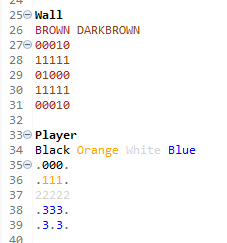
\includegraphics[width=0.50\textwidth]{images/Syntax_colouring.png}
%     \caption{Syntax highlighting}
%     \label{fig:ide_colouring}
% \end{figure}

The second feature is an outline view\dd. An outline view is a separate window the game designer can open to gain an overview of their game's contents. This feature allows the game designer to quickly navigate the file based on its contents. For instance, if a designer desires to return to the code for a specific object, they can simply click on that object's name in the outline. The outline improves the efficiency of the designer, especially as the file size grows. The outline we design provides an overview and a navigation shortcut for all major components of PuzzleScript. Tool designers can easily extend this outline to provide an overview of smaller components or to display additional data. Figure\ref{fig:ide_outline} shows this outline view with all branches expanded.

\begin{figure}[!t]
    \centering
    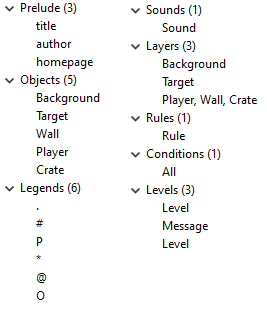
\includegraphics[width=0.5\textwidth]{images/Example_outline.png}
    \caption{IDE Outline}
    \label{fig:ide_outline}
\end{figure}

The third feature of the IDE is the display of error messages. In the original implementation, messages just appear in the console after compilation. However, this kind of implementation does not scale well with high number of messages. As such, we design ScriptButler's IDE so that it display the error messages right next to the code line creating the issue. Figure \ref{fig:ide_messages} shows this design implemented. The final feature of the IDE is a contextual menu. This contextual menu provides game designers with the ability to start up the Web GUI straight from the editor. However, the feature is very extensible and can be used for a wide variety of actions. For instance, it should be possible to use it to export the game or share it online. 

\begin{figure}[!t]
    \centering
    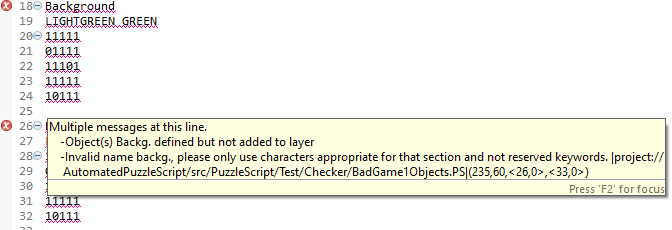
\includegraphics[width=0.85\textwidth]{images/Rascal_IDE.png}
    \caption{IDE Messages}
    \label{fig:ide_messages}
\end{figure}


In conclusion, ScriptButler's IDE provides game designers with an editor to interact with the tool itself. This editor supports game designers with a wide variety of features that make programming more efficient.



